\documentclass[12pt]{article}
\usepackage{graphicx}
\usepackage[margin=2cm]{geometry}
\usepackage[utf8]{inputenc}
\usepackage{tikz}
\usepackage[export]{adjustbox}
\usepackage{indentfirst}
\usepackage{wrapfig}
\usepackage{listings}
\usepackage{color}
\usepackage{enumerate}
\usepackage{amssymb, bm}
\usepackage{csvsimple}
\usepackage{tikz}
\usetikzlibrary{positioning}

\newcommand\tab[1][1cm]{\hspace*{#1}}
\definecolor{mygreen}{rgb}{0,0.6,0}
\definecolor{mygray}{rgb}{0.5,0.5,0.5}
\definecolor{mymauve}{rgb}{0.58,0,0.82}
\lstset{ %
    backgroundcolor=\color{gray!10!white},
  basicstyle=\tiny, %footnotesize,        % the size of the fonts that are used for the code
  breakatwhitespace=false,         % sets if automatic breaks should only happen at whitespace
  breaklines=true,                 % sets automatic line breaking
  captionpos=b,                    % sets the caption-position to bottom
  commentstyle=\color{mygreen},    % comment style
  deletekeywords={...},            % if you want to delete keywords from the given language
  escapeinside={\%*}{*)},          % if you want to add LaTeX within your code
  extendedchars=true,              % lets you use non-ASCII characters; for 8-bits encodings only, does not work with UTF-8
  frame=single,	                   % adds a frame around the code
  keepspaces=true,                 % keeps spaces in text, useful for keeping indentation of code (possibly needs columns=flexible)
  keywordstyle=\color{blue},       % keyword style
  language=Python,                 % the language of the code
  morekeywords={*,...},           % if you want to add more keywords to the set
  numbers=left,                    % where to put the line-numbers; possible values are (none, left, right)
  numbersep=10pt,                   % how far the line-numbers are from the code
  numberstyle=\tiny\color{mygray}, % the style that is used for the line-numbers
  rulecolor=\color{black},         % if not set, the frame-color may be changed on line-breaks within not-black text (e.g. comments (green here))
  showspaces=false,                % show spaces everywhere adding particular underscores; it overrides 'showstringspaces'
  showstringspaces=false,          % underline spaces within strings only
  showtabs=false,                  % show tabs within strings adding particular underscores
  stepnumber=1,                    % the step between two line-numbers. If it's 1, each line will be numbered
  stringstyle=\color{mymauve},     % string literal style
  tabsize=1,	                   % sets default tabsize to 2 spaces
  title=\lstname                   % show the filename of files included with \lstinputlisting; also try caption instead of title
}
\graphicspath{ }
\usetikzlibrary{arrows}

\title{\textbf{COMP0086 Summative Assignment}}
%\author{Jian Shu (James) Wu \\ }
\date{Nov 14, 2022}

\begin{document}
\maketitle
\section*{Question 1}


\begin{enumerate}

\item[(a)] Our sample space for images is $\{0, 1\}^D$, a binary space with $D$ dimensions, the number of pixels in the image.
Thus, picking the exponential family best suited on this sample space is the D-dimensional multivariate Bernoulli distribution which shares the same sample space.
On the other hand, a D-dimensional multivariate Gaussian has the sample space $\mathbb{R}^D$, which does not match the sample space of our data.
To match our data sample space, we would have to define additional mapping between our data and model spaces which adds unnecessary complexity.
Thus it would be inappropriate to model this dataset of images with a multivariate Gaussian.

\item[(b)] For $\mathcal{D} := \{x^{(n)}\}_{n=1}^N$ a data set of N images, the joint likelihood (assuming images are independently and identically distributed) is the product of N D-dimensional multivariate Bernoulli distributions, one for each image:

$$P(\mathcal{D}|\textbf{p}) = \prod_{n=1}^N P(x^{(n)} | \textbf{p})$$


Substituting the D-dimensional multivariate Bernoulli:

$$P(\mathcal{D}|\textbf{p}) = \prod_{n=1}^{N}\prod_{d=1}^{D} p_d^{x_d^{(n)}} (1-p_d)^{1-x_d^{(n)}}$$

Taking the logarithm of this, we get the log likelihood:

$$\mathcal{L}(\mathcal{D}|\textbf{p}) = \sum_{n=1}^{N}\sum_{d=1}^{D} [x_d^{(n)}\log(p_d) +  (1-x_d^{(n)})\log(1-p_d)]$$

Note that since the logarithm of the mean is a monotonic increasing function on $\mathbb{R}_+$, the maximisers and minimisers of the likelihood do not change.

To solve for the maximum likelihood estimate, $\hat p_d$, we can take the derivative of $\mathcal{L}(\mathcal{D}|\textbf{p})$ with respect to $p_d$, the $d^{th}$ element of $\textbf{p}$:

$$\frac{\partial\mathcal{L}(\mathcal{D}|\textbf{p})}{\partial p_d} = \sum_{n=1}^{N} (\frac{x_d^{(n)}}{p_d} -  \frac{1-x_d^{(n)}}{1-p_d})$$
$$\frac{\partial\mathcal{L}(\mathcal{D}|\textbf{p})}{\partial p_d} = \frac{\sum_{n=1}^{N} x_d^{(n)}}{p_d} -  \frac{\sum_{n=1}^{N} (1-x_d^{(n)})}{1-p_d}$$

and set the derivative to zero and solve for $\hat p_d$:

$$\frac{\sum_{n=1}^{N} x_d^{(n)}}{\hat p_d} -  \frac{\sum_{n=1}^{N} (1-x_d^{(n)})}{1-\hat p_d} = 0$$
$$ \sum_{n=1}^{N} x_d^{(n)} - \hat p_d\sum_{n=1}^{N} x_d^{(n)} - \hat p_d  \cdot N + \hat p_d \sum_{n=1}^{N}x_d^{(n)} = 0$$
$$  \hat p_d = \frac{1}{N}\sum_{n=1}^{N} x_d^{(n)}$$

Moreover, the second derivative with respect to $p_d$:

$$\frac{\partial\mathcal{L}(\mathcal{D}|\textbf{p})}{\partial p_d^2} = \frac{-\sum_{n=1}^{N} x_d^{(n)}}{p_d^2} +  \frac{-\sum_{n=1}^{N} (1-x_d^{(n)})}{(1-p_d)^2}$$

For a maximum, we need to show that the second derivative is negative.
Since $x_d^{(n)} \in \{0, 1\}$, in the worst case, of $N=1$, the single pixel must either be white ($\sum_{n=1}^{N} > 0$) or black ($\sum_{n=1}^{N} 1-x_d^{(n)} > 0$) so $\frac{\partial\mathcal{L}(\mathcal{D}|\textbf{p})}{\partial p_d^2} < 0$ will be guaranteed and $\hat p_d$ is a maximum as required for the maximum likelihood estimate.

Because we assume that each pixel is independent (we are taking the product of D one dimensional Bernoulli distributions), we can express the maximum likelihood for $\textbf{p}$ in matrix form as $\hat \textbf{p}$:

$$\hat \textbf{p} = \frac{1}{N}\sum_{n=1}^{N} \textbf{x}^{(n)}$$

%\item[(c)] Assuming independent Beta priors on the parameters $p_d$:
%
%$$P(p_d) = \frac{1}{B(\alpha, \beta)} p^{\alpha-1}_d (1-p_d)^{\beta-1}$$
%
%and $P(\textbf{p}) = \prod_d P(p_d)$ Find the maximum a posteriori (MAP) estimator for \textbf{p}. [5 marks]

\item[(c)] From Bayes' Theorem:

$$P(\textbf{p}|\mathcal{D}) = \frac{ P(\mathcal{D}|\textbf{p})P(\textbf{p})}{P(\mathcal{D})}$$

Taking the logarithm:

$$\mathcal{L}(\textbf{p}|\mathcal{D}) = \mathcal{L}(\mathcal{D}|\textbf{p})+ \mathcal{L}(\textbf{p}) - \mathcal{L}(\mathcal{D})$$

Taking the derivative with respect to $p_d$:

$$\frac{\partial\mathcal{L}(\textbf{p}|\mathcal{D})}{\partial p_d} = \frac{\partial\mathcal{L}(\mathcal{D}|\textbf{p})}{\partial p_d} + \frac{\partial\mathcal{L}(\textbf{p})}{\partial p_d}$$

where $\frac{\partial\mathcal{L}(\mathcal{D})}{\partial p_d}$=0 because it doesn't depend on $p_d$.

We know (b):

$$\frac{\partial\mathcal{L}(\mathcal{D}|\textbf{p})}{\partial p_d} = \frac{\sum_{n=1}^{N} x_d^{(n)}}{p_d} -  \frac{\sum_{n=1}^{N} (1-x_d^{(n)})}{1-p_d}$$

For the second term $\frac{\partial\mathcal{L}(\textbf{p})}{\partial p_d}$, we start with $P(\textbf{p}))$:

$$P(\textbf{p})) = \prod_{d=1}^D P(p_d)$$

Assuming independent Beta priors on the parameters $p_d$:

$$P(\textbf{p}) = \prod_{d=1}^D \frac{1}{B(\alpha, \beta)} p^{\alpha-1}_d (1-p_d)^{\beta-1}$$

Taking the logarithm:

$$\mathcal{L}(\textbf{p}) = \sum_{d=1}^{D} -\log (B(\alpha, \beta)) + (\alpha-1)\log p_d + (\beta-1)\log(1-p_d)$$

Taking the derivative with respect to $p_d$:

$$\frac{\partial\mathcal{L}(\textbf{p})}{\partial p_d} = -\log (B(\alpha, \beta)) + (\alpha-1)\log p_d + (\beta-1)\log(1-p_d))$$

Since we are only concerned with $p_d$, we are only left with a single element of the summation pertaining to $p_d$.

Simplifying:

$$\frac{\partial\mathcal{L}(\textbf{p})}{\partial p_d} = \frac{(\alpha-1)}{p_d} -  \frac{(\beta-1)}{1-p_d}$$

Combining to have an expression for the log posterior derivative $\frac{\partial\mathcal{L}(\textbf{p}|\mathcal{D})}{\partial p_d}$:

$$\frac{\partial\mathcal{L}(\textbf{p}|\mathcal{D})}{\partial p_d} = \frac{\sum_{n=1}^{N} x_d^{(n)}}{p_d} -  \frac{\sum_{n=1}^{N} (1-x_d^{(n)})}{1-p_d} + \frac{(\alpha-1)}{p_d} -  \frac{(\beta-1)}{1-p_d}$$
$$\frac{\partial\mathcal{L}(\textbf{p}|\mathcal{D})}{\partial p_d} = \frac{(\alpha-1) + \sum_{n=1}^{N} x_d^{(n)}}{p_d} -  \frac{(\beta-1) + \sum_{n=1}^{N} (1-x_d^{(n)})}{1-p_d}$$


To find the maximum a posteriori (MAP) estimate $\hat{p_d}$ with $\frac{\partial\mathcal{L}(\textbf{p}|\mathcal{D})}{\partial p_d} = 0$:

$$0 = \frac{(\alpha-1) + \sum_{n=1}^{N} x_d^{(n)}}{\hat{p_d}} -  \frac{(\beta-1) + \sum_{n=1}^{N} (1-x_d^{(n)})}{1-\hat{p_d}}$$
$$0 = (1-\hat{p_d})(\alpha-1) + (1-\hat{p_d})\bigg(\sum_{n=1}^{N} x_d^{(n)}\bigg) -  \hat{p_d}(\beta-1) - \hat{p_d}\bigg(\sum_{n=1}^{N} (1-x_d^{(n)})\bigg)$$
$$0 = (\alpha-\alpha \hat{p_d} + \hat{p_d} - 1) +\bigg(\sum_{n=1}^{N} x_d^{(n)} - \hat{p_d} \sum_{n=1}^{N} x_d^{(n)}\bigg) -  (\hat{p_d}\beta-\hat {p_d}) - \bigg(\hat{p_d}\cdot N - \hat{p_d}\sum_{n=1}^{N}x_d^{(n)}\bigg)$$

Cancelling the $\hat p_d\sum_{n=1}^{N} x_d^{(n)}$ terms:

$$0 = \alpha-\alpha \hat{p_d} + \hat{p_d} - 1 +\sum_{n=1}^{N} x_d^{(n)} -  \hat{p_d}\beta+\hat{p_d} - \hat{p_d}\cdot N$$
$$0 = \hat{p_d}(2-\alpha-\beta-N) + \alpha - 1 +\sum_{n=1}^{N} x_d^{(n)}$$
$$\hat{p_d} =  \frac{\alpha - 1 +\sum_{n=1}^{N} x_d^{(n)}}{(N+\alpha+\beta-2)}$$

To show that this is a maximum, the second derivative is:

$$\frac{\partial^2\mathcal{L}(\textbf{p}|\mathcal{D})}{(\partial p_d)^2} = \frac{(1-\alpha) - \sum_{n=1}^{N} x_d^{(n)}}{(p_d)^2} +  \frac{(1-\beta) - \sum_{n=1}^{N} (1-x_d^{(n)})}{(1-p_d)^2}$$.

For a maximum, we need $\frac{\partial^2\mathcal{L}(\textbf{p}|\mathcal{D})}{(\partial p_d)^2} < 0$ meaning that we need at least one of the strict inequalities $\alpha < 1- \sum_{n=1}^{N} x_d^{(n)}$ or $\beta < 1-\sum_{n=1}^{N} (1-x_d^{(n)})$ to be satisified, where the other can be $\leq$. The Beta distribution requires $\alpha > 0$ and $\beta > 0$ so this requirement will always be satisfied (in the worst case of a single image, either $x_d^{(1)}=1$ or $1-x_d^{(1)}=1$).






Due to independence of our likelihood and priors for each dimension, we can express the maximum a priori for \textbf{p} in matrix form as \hat \textbf{p}:

$$\hat \textbf{p} =   \frac{\alpha - 1 +\sum_{n=1}^{N} \textbf{x}^n}{(N+\alpha+\beta-2)}$$


\newpage
\item[(d\&e)] The Python code for MLE and MAP:
\lstinputlisting[language=Python, caption: MLE and MAP Implementation,]{src/solutions/q1.py}
\newpage
%  \begin{figure}[h]
%  \centering
%  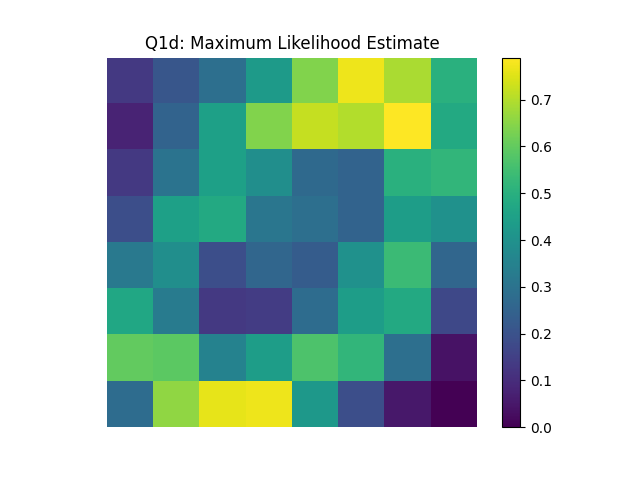
\includegraphics[scale=0.5]{outputs/q1/q1d}
%  \caption{ML parameters}
%  \label{fig:1d}
%  \end{figure}
%  \begin{figure}[h]
%  \centering
%  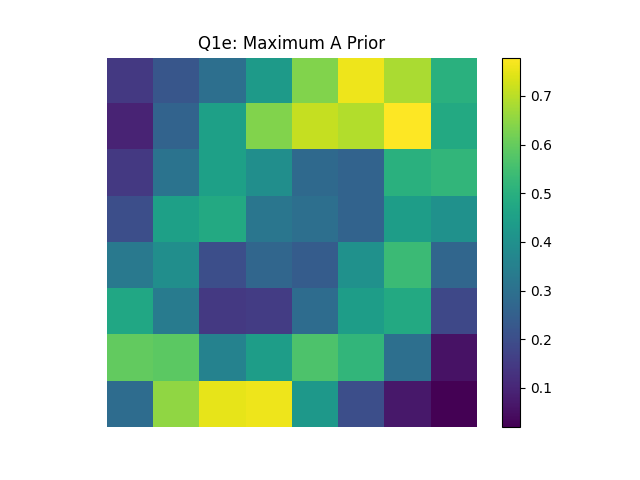
\includegraphics[scale=0.5]{outputs/q1/q1e}
%  \caption{MAP parameters}
%  \label{fig:1e}
%  \end{figure}

Displaying the learned parameters:
\begin{figure}[h]
\centering
\begin{minipage}{0.5\textwidth}
  \centering
  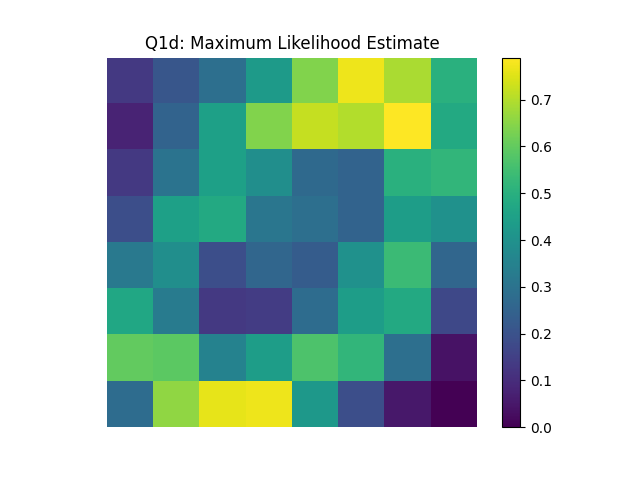
\includegraphics[scale=0.5]{outputs/q1/q1d}
  \caption{ML parameters}
  \label{fig:1d}
\end{minipage}%
\begin{minipage}{0.5\textwidth}
  \centering
  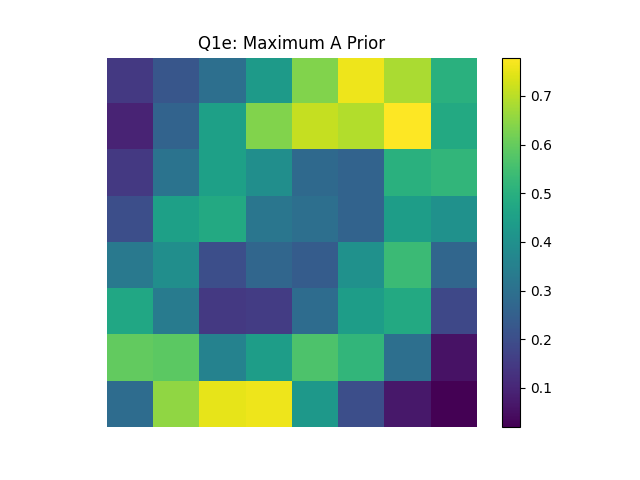
\includegraphics[scale=0.5]{outputs/q1/q1e}
  \caption{MAP parameters}
  \label{fig:1e}
\end{minipage}
\end{figure}

Comparing the equations:

    $$\hat{\textbf{p}}^{MLE} = \frac{1}{N}\sum_{n=1}^{N} \textbf{x}^{(n)}$$

    and

    $$\hat{\textbf{p}}^{MAP}  =  \frac{\alpha - 1 +\sum_{n=1}^{N} \textbf{x}^n}{(N+\alpha+\beta-2)}$$


We see that when the number of data points increases, the MAP estimate approaches $\frac{1}{N}\sum_{n=1}^{N} \textbf{x}^{(n)}$, the MLE. This result makes sense because as our data set gets bigger, are less reliant on our prior.  Moreover, if in our data set of images, a specific pixel in all of these images are white or all black, the MLE for that pixel will be binary. This may not be be representative of our intuitions about images, where there should be some non-zero probability of a pixel being black or white. Thus, introducing an appropriate prior will ensure that the probability of that pixel will never be zero or one. Moreover, a prior can also help ensure numerical stability during calculations. The logarithm of zero is negative infinity, so having probability zero can be problematic for log-likelihoods calculations. A prior can ensure non-zero probabilities. In our case, by using a small Beta distribution prior on each pixel, our parameter values are biased be close to 0.5 and to never be at the extremities 0 and 1. We can see this in our MAP parameters figure where the range of our parameters is smaller than the range for the ML parameters. Also, the MLE has values of zero whereas the MAP does not. Interestingly, when $\alpha=1$ and $\beta=1$, $\hat{\textbf{p}}^{MLE} = \hat{\textbf{p}}^{MAP}$, intuitively this is when the prior is a uniform distribution and so there aren't any biases on the location of $\textbf{p}$ and we recover the MLE. On the other hand, a misspecified prior can be problematic, as the estimated parameters might be skewed by the prior and not properly represent the underlying data generating process and this can be worse than using the MLE.
%In this example, we're using images of different digits as part of our data set. If a particular digit occurs more frequently in the data set, we will see that digit when visualising the MLE or MAP (the digit zero in this case), they simply provides the "average" image pixels. With a set of images with more equal representation of each digit, the parameter visualisation could be an image overlaying the different digits, which is not representative of the "most likely" image in the data. In this case where our data is likely clustered, using a multimodal likelihood is probably a better idea than the unimodal likelihood we've used.

    We can also visualise $\hat{\textbf{p}}^{MAP}-\hat{\textbf{p}}^{MLE}$ to see that for likelihoods greater than 0.5 in the MLE, the MAP has a lower value and for likelihoods less than 0.5, the MAP has a higher value, confirming our intutions.

  \end{figure}
  \begin{figure}[h]
  \centering
  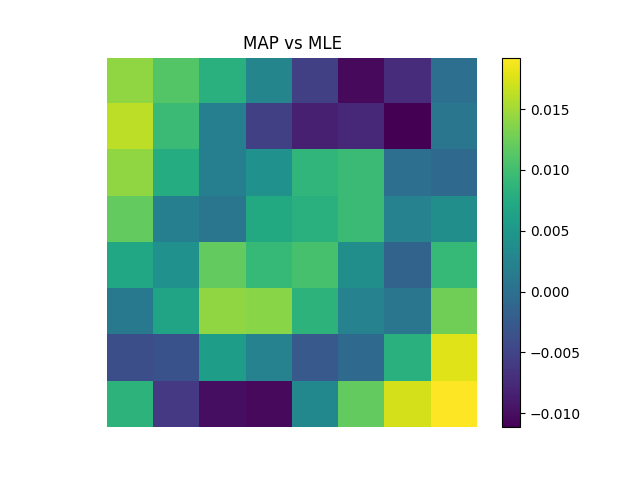
\includegraphics[scale=0.5]{outputs/q1/q1e-mle-vs-map}
  \caption{$\hat{\textbf{p}}^{MAP}-\hat{\textbf{p}}^{MLE}$}
  \label{fig:1e}
  \end{figure}

%With MAP, if we have priors skewed towards the parameters for under represented digits in our data, it is more likely to "even out" the estimated parameters. In our case, we used the same Beta prior on all pixels, essentially placing a "uniform shading" on the entire image, so we could not




\end{enumerate}

\newpage

\section*{Question 2}


\begin{enumerate}

\item[(a)] When all D components are generated from a Bernoulli distribution with $p_d = 0.5$, we have the likelihood function for model $M_1$:

$$P(\textbf{x}^{(n)|\textbf{p}^{(1)}}=[0.5, 0.5,...,0.5]^T) = \prod_{d=1}^{D} (0.5)^{x_d^{(n)}} (0.5)^{1-x_d^{(n)}}$$

\item[(b)] When all D components are generated from Bernoulli distributions with unknown, but identical, $p_d$, we have the likelihood function for model $M_2$:

$$P(\textbf{x}^{(n)}|\textbf{p}^{(2)}}=[p_d, p_d, ..., p_d]^T) = \prod_{d'=1}^{D} p_d^{x_{d'}^{(n)}} (1-p_d)^{1-x_{d'}^{(n)}}$$


\item[(c)] When each component is Bernoulli distributed with separate, unknown $p_d$, we have the likelihood function for model $M_3$:

$$P(\textbf{x}^{(n)}|\textbf{p}^{(3)}}=[p_1, p_2, ..., p_D]^T) = \prod_{d=1}^{D} p_d^{x_d^{(n)}} (1-p_d)^{1-x_d^{(n)}}$$



For each model $M_i$, we can marginalise out $P$ to get $P( \{\textbf{x}^{(n)}\}_{n=1}^{N}|M_i)$:

$$P( \{\textbf{x}^{(n)}\}_{n=1}^{N}|M_i) = \int_0^1...\int_0^1 P( \{\textbf{x}^{(n)}\}_{n=1}^{N}|p_d, M_i)P(p_d|M_i) dp_1...dp_D$$

where $d=1,...,D$ and $ \{\textbf{x}^{(n)}\}_{n=1}^{N}$ is our data set.

Given that the prior of any unknown probabilities is uniform, i.e. $P(p_d | M_i) = 1$. We can simplify:

$$P( \{\textbf{x}^{(n)}\}_{n=1}^{N}|M_i) = \int_0^1...\int_0^1 P(\{\textbf{x}^{(n)}\}_{n=1}^{N}|p_d, M_i) dp_1...dp_D$$

For $M_1$, we have that all pixels have probability 0.5:

$$P( \{\textbf{x}^{(n)}\}_{n=1}^{N}|M_1) = \int_0^1...\int_0^1 \prod_{j=n}^{N} \prod_{d=1}^{D} (0.5)^{x_d^{(n)}} (1-0.5)^{1-{x_d}^{(n)}} d\theta_1...d\theta_D$$

We can remove the integrals and knowing that either $x_d^{(n)}$ or $1-x_d^{(n)}$ will be 1 and the other zero, we can simplify $(0.5)^{x_d^{(n)}} (1-0.5)^{1-{x_d}^{(n)}}$ to $0.5$:

$$P( \{\textbf{x}^{(n)}\}_{n=1}^{N}|M_1) = \prod_{j=1}^{N} \prod_{d=1}^D (0.5)$$
$$P( \{\textbf{x}^{(n)}\}_{n=1}^{N}|M_1) = (0.5)^{N\cdot D}$$

For $M_2$, we have that all pixels share some probability $p_d$ so we only need to integrate over a single variable $p_d$:

$$P( \{\textbf{x}^{(n)}\}_{n=1}^{N}|M_2) = \int_0^1 \prod_{n=1}^{N} \prod_{d'=1}^D p^{x_{d'}^{(n)}} (1-p_d)^{1-{x_{d'}}^{(n)}} dp_d$$

Changing the products to sums:

$$P( \{\textbf{x}^{(n)}\}_{n=1}^{N}|M_2) = \int_0^1  p_d^{\sum_{n=1}^{N} \sum_{d'=1}^D x_{d'}^{(n)}} (1-p)^{\sum_{j=1}^{N} \sum_{d'=1}^D 1-{x_{d'}^{(n)}}} d p_d$$

Rewriting:

$$P( \{\textbf{x}^{(n)}\}_{n=1}^{N}|M_2) = \int_0^1  p_d^{k} (1- p_{d'=1})^{N\cdot D-k} d p_d$$

where $k =\sum_{n=1}^{N} \sum_{d'=1}^D x_{d'}^{(n)}$.

This integral is the beta function:

$$P( \{\textbf{x}^{(n)}\}_{n=1}^{N}|M_2) = \frac{k! (N\cdot D-k)!}{(N\cdot D+1)!}$$

For $M_3$, we need an integral for each $p_d$:

$$P( \{\textbf{x}^{(n)}\}_{n=1}^{N}|M_3) = \int_0^1 ... \int_0^1 \prod_{n=1}^{N} \prod_{d=1}^D  p_d^{x_d^{(n)}} (1- p_d)^{1-{x_d}^{(n)}} d p_1 ... d p_D$$

We can separate the integrals to only contain the relevant $p_d$:

$$P( \{\textbf{x}^{(n)}\}_{n=1}^{N}|M_3) = \prod_{d=1}^D \Bigg( \int_0^1 \prod_{n=1}^{N}   p_d^{x_d^{(n)}} (1- p_d)^{1-{x_d}^{(n)}} d p_d \Bigg)$$

Changing the products to sums:

$$P( \{\textbf{x}^{(n)}\}_{n=1}^{N}|M_3) = \prod_{d=1}^D \Bigg( \int_0^1   p_d^{\sum_{n=1}^{N} x_d^{(n)}} (1- p_d)^{\sum_{n=1}^{N} 1-{x_d}^{(j)}} d p_d \Bigg)$$

In this case, we have the product of integrals where each evaluates to a beta function:

$$P( \{\textbf{x}^{(n)}\}_{n=1}^{N}|M_3) = \prod_{d=1}^D \frac{k_d! (N-k_d)!}{(N+1)!}$$

where $k_d = \sum_{n=1}^{N} x_d^{(in}$.

The posterior probability of a model $M_i$ can be expressed:

$$P(M_i |  \{\textbf{x}^{(n)}\}_{n=1}^{N}) = \frac{P( \{\textbf{x}^{(n)}\}_{n=1}^{N}|M_i)P(M_i)}{P( \{\textbf{x}^{(n)}\}_{n=1}^{N})}$$

We only ave three models, so in this case the normalisation $P(D)$ can be expressed as a sum:

$$P(M_i| \{\textbf{x}^{(n)}\}_{n=1}^{N}) = \frac{P( \{\textbf{x}^{(n)}\}_{n=1}^{N}|M_i)P(M_i)}{\sum_{i\in \{1,2,3\}} P( \{\textbf{x}^{(n)}\}_{n=1}^{N}|M_i)P(M_i)}$$

Given that $P(M_i) = \frac{1}{3}$ for all $i \in \{1,2,3\}$:

$$P(M_i| \{\textbf{x}^{(n)}\}_{n=1}^{N}) = \frac{P( \{\textbf{x}^{(n)}\}_{n=1}^{N}|M_i)}{\sum_{i\in \{1,2,3\}} P( \{\textbf{x}^{(n)}\}_{n=1}^{N}|M_i)}$$


Calculating the posterior probabilities of each of the three models having generated the data in binarydigits.txt using python we can show the values in the table below:

\begin{center}
\begin{tabular}{l|c}%
 \bfseries $i$ & \bfseries$ P(M_i|\mathcal{D})$% specify table head
\csvreader[head to column names]{outputs/q2/q2c.csv}{}% use head of csv as column names
{\\\hline\csvcoli&\csvcolii}% specify your coloumns here
\end{tabular}
\end{center}

% TODO

\newpage
The Python code for calculating the posterior probabilities of the three models:
\lstinputlisting[language=Python]{src/solutions/q2.py}
\end{enumerate}
\newpage
\section*{Question 3}

\begin{enumerate}

%\item[(a)] Write down the likelihood for a model consisting of a mixture of K multivariate Bernoulli
%distributions. Use the parameters $\pi_1, . . . , \pi_K$ to denote the mixing proportions $(0 \leq \pi_k \leq 1; \sum_k \pi_k = 1)$ and arrange the K Bernoulli parameter vectors into a matrix P with elements
%$p_{kd}$ denoting the probability that pixel d takes value 1 under mixture component k. Assume the images are iid under the model, and that the pixels are independent of each other within each component distribution. [5 marks]
%
%
%Just as we can for a mixture of Gaussians, we can formulate this mixture as a latent variable
%model, introducing a discrete hidden variable $s(n) \in \{1, . . . , K \}$ where $P (s(n) = k|\pi) = \pi_k$.

\item[(a)] The likelihood for a model consisting of a mixture of K multivariate Bernoulli distributions can be expressed as the product across $N$ data points:

$$P(\{\textbf{x}^{(n)}\}_{n=1}^{N}|\theta) = \prod_{i=1}^{N}P(x_i|\theta)$$

where $\{\textbf{x}^{(n)}\}_{n=1}^{N}$ is our data set with $\textbf{x}^{(n)} \in \mathbb{R}^{D \times 1}$ and $\theta = \{\pi, \mathbf{P}\}$, $\pi = [\pi_1, . . . , \pi_K] \in \mathbb{R}^{K \times 1}$$ our mixing proportions $(0 \leq \pi_k \leq 1; \sum_k \pi_k = 1)$ and $\mathbf{P} \in \mathbb{R}^{D \times K}$ the K Bernoulli parameter vectors with elements $p_{kd}$ denoting the probability that pixel d takes value 1 under mixture component k. We are also the images are iid under the model, and that the pixels are independent of each other within each component distribution.

For each $P(\textbf{x}^{(n)}|\theta)$:

$$P(\textbf{x}^{(n)}|\theta) = \sum_{k=1}^{K} \pi_k \prod_{d=1}^D (p_{kd})^{\textbf{x}^{(n)}_{d}} (1-p_{kd})^{1-\textbf{x}^{(n)}_{d}}$$

The log-likelihood $\mathcal{L}(\textbf{x}^{(n)}|\theta)$ can be expressed in matrix form:

$$\mathcal{L}(\textbf{x}^{(n)}|\theta) = \log \sum_{k=1}^{K}  \pi_k \exp\bigg(\textbf{x}^{(n)}\log(\mathbf{P}_{k}) + (1-\textbf{x}^{(n)})\log(1-\mathbf{P}_{k})\bigg) $$

which can be further vectorised using Python scipy's $logsumexp$ operation.

Moreover, the log-likelihood $\mathcal{L}(\{\textbf{x}^{(n)}\}_{n=1}^{N}|\theta)$ can be expressed:

$$\mathcal{L}(\{\textbf{x}^{(n)}\}_{n=1}^{N}|\theta) = \sum_{i=1}^{N} \Bigg( \log \sum_{k=1}^{K}  \pi_k \exp\bigg(\textbf{x}^{(n)}\log(\mathbf{P}_{k}) + (1-\textbf{x}^{(n)})\log(1-\mathbf{P}_{k})\bigg) \Bigg)$$

\item[(b)] The expression for the responsibility of mixture component k for data vector
$x^{(n)}$, i.e. $r_{nk} \equiv P (s^{(n)} = k|x^{(n)}, \pi, \mathbf{P})$. This computation provides the E-step for an EM algorithm.

We know that:

$$P(A|B) \propto P(B|A)P(A)$$

Thus,


$$P(s^{(n)} = k|x^{(n)}, \pi, \mathbf{P}) \propto  P(x^{(n)} | s^{(n)} = k, \pi, \mathbf{P}) P(s^{(n)} = k|\pi, \mathbf{P})$$

where $s^{(n)} \in \{1,...,K\}$ a discrete latent variable where $P(s^{(n)} = k|x^{(n)} | \pi) = \pi_k$. Note that $P(s^{(n)} = k|x^{(n)} | \pi) = P(s^{(n)} = k|x^{(n)} | \pi, \mathbf{P})$ as $s^{(n)$ isn't dependent on $\mathbf{P}$.

Let $P(s^{(n)} = k|x^{(n)}, \pi, \mathbf{P}) \propto P(s^{(n)}$ be the unnormalised responsibility $\tilde{r}_{nk}$. Using the mixture for component $k$ and the likelihood function of component $k$:

$$\tilde{r}_{nk} = \pi_k \prod_{d=1}^D (p_{kd})^{x^{(n)}_{d}} (1-p_{kd})^{1-x^{(n)}_{d}}$$

Normalising across the components:

$$r_{nk} = \frac{\tilde{r}_{nk}}{\sum_{j=1}^K\tilde{r}_{nj}}$$

and $r_{nk}$, we have calculated $P(s^{(n)} = k|x^{(n)}, \pi, \mathbf{P})$ for the E step.

Moreover,

$$ \log \tilde{r}_{nk} = \log \pi_k + \sum_{d=1}^D \bigg( x^{(n)}_{d}\log(p_{kd}) + (1-x^{(n)}_{d}) \log(1-\exp(\log(p_{kd}))) \bigg)$$

and

$$\log r_{nk} = \log\tilde{r}_{nk} - \log\sum_{j=1}^K\exp(\log\tilde{r}_{nj})$$

which can be vectorised using Python scipy's $logsumexp$ operation.



\item[(c)] We know that the expectation log joint can be expressed:

$$\Bigg\langle \sum_n \log P(x^{(n)}, s^{(n)}| \pi, \mathbf{P})\Bigg\rangle_{q(\{s^{(n)}\})} = \sum_{n=1}^N q(s^{(n)}) \log P(x^{(n)}, s^{(n)}| \pi, \mathbf{P})$$

Let this quantity be $E$.

Filling in the appropriate quantities:

$$ E = \sum_n r_n^T[\log(\pi)+\log(\mathbf{P})^T x^{(n)} + \log(1-\mathbf{P})^T(1-x^{(n)})]$$

where $q(s^{(n)}) = r_n^T$ and $\log P(x^{(n)}, s^{(n)}) = \log(\pi)+\log(\mathbf{P})^T x^{(n)} + \log(1-\mathbf{P})^T(1-x^{(n)})$. Noting that $P(x^{(n)}, s^{(n)}| \pi, \mathbf{P}) = P(x^{(n)}|s^{(n)}) \pi, \mathbf{P}) P(s^{(n)})| \pi, \mathbf{P}) = \tilde{r}_{n}$

To maximise with respect to $\pi$ and $P$ for the M step, we want to take the derivative, set to zero, and solve for $\hat\pi$ and $\hat P$.

For the $k^{th}$ element of $\pi$:

$$\frac{\partial E}{\partial \pi_k} = \sum_n r_{nk} \frac{1}{\pi_m}$$

and

$$\frac{\partial E}{\partial \pi_k} + \lambda = 0$$

where $\lambda$ is a Lagrange multiplier ensuring that the mixing proportions sum to unity.

Thus,

$$\hat \pi_m = \frac{1}{N}\sum_{n}r_{nk}$$

For the $dk^{th}$ element of P:

$$\frac{\partial E}{\partial P_{dk}} = \sum_n r_{nk}\frac{\partial}{\partial P_{dk}}[x^{(n)}_{d}\log P_{dk}+(1-x^{(n)}_{d}) \log(1-P_{dk})]$$

Simplying:

$$\frac{\partial E}{\partial P_{dk}} = \sum_n r_{nk}(\frac{x^{(n)}_{d}}{ P_{dk}}-\frac{1-x^{(n)}_{d}}{1-P_{dk}})$$

Setting the derivative to zero:

$$\frac{\sum_n  x^{(n)}_{d}r_{nk}}{ P_{dk}}-\frac{\sum_n r_{nk}-\sum_n  x^{(n)}_{d}r_{nk}}{1-P_{dk}} = 0$$

Solving for $P_{dk}$:

$$P_{dk}\sum_n r_{nk}-P_{dk}\sum_n x^{(n)}_{d}r_{nk} = \sum_n  x^{(n)}_{d}r_{nk}-P_{dk}\sum_n  x^{(n)}_{d}r_{nk}$$

Thus,

$$\hat{P}_{dk} = \frac{\sum_n x^{(n)}_{d}r_{nk}}{\sum_n r_{nk}}$$

We have the maximizing parameters for the expected log-joint

$$\arg \max_{\pi, P} \Bigg\langle \sum_n \log P(x^{(n)}, s^{(n)}| \pi, P)\Bigg\rangle_{q(\{s^{(n)}\})}$$

thus obtaining an iterative update for the parameters $\pi$ and $P$ in the M-step of EM.

\newpage
\item[(d)] The Python code for the EM algorithm:
\lstinputlisting[language=Python]{src/solutions/q3.py}
\newpage
Run your algorithm on the data set for values of K in {2, 3, 4, 7, 10}. Plot the log likelihood as a function of the iteration number, and display the parameters found. [30 marks]


\item[(e)] Run the algorithm a few times starting from randomly chosen initial conditions. Do you obtain the same solutions (up to permutation)? Does this depend on K? Show the learned probability vectors as images.

Comment on how well the algorithm works, whether it finds good clusters (look at the cluster means and responsibilities and try to interpret them), and how you might improve the model. [10 marks]

\end{enumerate}

\newpage
\section*{Question 5}

\begin{enumerate}

%\item[] \textbf{[70 points] Decrypting Messages with MCMC.} You are given a passage of English text that has been encrypted by remapping each symbol to a (usually) different one. For example,
%
%$$a \rightarrow s$$
%$$b \rightarrow !$$
%$$\langle space \rangle \rightarrow v$$
%$$\cdots$$
%
%Thus a text like ‘a boy. . . ’ might be encrypted by ‘sv!op. . . ’. Assume that the mapping between symbols is one-to-one. The file symbols.txt gives the list of symbols, one per line (the second line is 〈space〉). The file message.txt gives the encrypted message.
%
%Decoding the message by brute force is impossible, since there are 53 symbols and thus 53! possible permutations to try. Instead we will set up a Markov chain Monte Carlo sampler to find modes in the space of permutations.
%
%We model English text, say $s_1s_2\cdots s_n$ where $s_i$ are symbols, as a Markov chain, so that each symbol is independent of the preceding text given only the symbol before:

%$$p(s_1s_2\cdots s_n) = p(s_1)\prod_{i=2}^{n}p(s_i|s_{i-1})$$

\item[(a)] Let $p(\textbf{s}_i,\textbf{s}_{i-1})$ be the probability of the pair of symbols $\textbf{s}_i$ and $\textbf{s}_{i-1}$ occurring together in the text ($\textbf{s}_{i-1}$ followed by $\textbf{s}_i$ where order matters).
We can model $p(\textbf{s}_i,\textbf{s}_{i-1})$ as a multinomial distribution with $N=1$ and $D=53^2$:

$$p(\textbf{s}_i,\textbf{s}_{i-1}) = \frac{1}{s^1! s^2! \cdots s^{53^2}} \prod_{j \in \{1,...53\}, k \in \{1,...53\}} p_{s_i, s_{i-1}}^{t^{s_i, s_{i-1}}}$$

where $t^{s_i, s_{i-1}}$ is an indicator of transition $s_{i-1}$ to $s_i$.
For convenience we will denote $t^{(\alpha, \beta)})$ as the transition from
A multinomial distribution is appropriate because there can only be only one of 53 symbols chosen as $s$ (i.e. a 53 dimensional dice).
Thus, $p(s=s_i)$ represents the probability of the symbol $s_i$ in the text.

We can convert p(s) into exponential family form:

$$p(\textbf{s}) = \frac{1}{s^1! s^2! \cdots s^D} \exp{(\textbf{s}^T \log(\textbf{p}))}$$

where $\textbf{p}$ is the vector of $p_i$'s.
Thus the sufficient statistic is $T(\textbf{s}) = \textbf{s}^T$.

The ML estimate

%Learn the transition statistics of letters and punctuation in English: Download a large text [say the English translation of War and Peace] from the web and estimate the transition probabilities $p(s_i = \alpha|s_{i-1} = \beta) := \Psi(\alpha, \beta)$, as well as the stationary distribution $\lim_{i\rightarrow \infty} p(s_i = \gamma) := \phi(\gamma)$. Assume that the first letter of your text (and also that of the encrypted text provided) is itself sampled from the stationary distribution. Give formulae for the ML estimates of these probabilities as functions of the counts of numbers of occurrences of symbols and pairs of symbols.
%Compute the estimated probabilities. Report the values as a table. [6 marks]







\item[(b)] The latent variables $\sigma(s)$ for different symbols $s$ are not independent.
This is because by choosing an encoding for one symbol $e = \sigma(s)$, the encoding for a second symbol $\sigma(s')$ cannot be $e$.
We have 53 symbols but only 52 degrees of freedom, because once we have defined the encoding for 52 symbols, the encoding for the $53^{rd}$ symbol cannot be chosen.
Thus, there exists a dependence between the symbols for a given $\sigma$.

The joint probability of the encrypted text $e_1 e_2 \cdots e_n$ given $\sigma$:

$$P(e_1, e_2,...,e_n|\sigma) = \psi(\gamma=\sigma^{-1}(e_1))\prod_{i=2}^n \psi(\alpha=\sigma^{-1}(e_i), \beta=\sigma^{-1}(e_{i-1}))$$

because $\sigma$ is the encoding function, mapping to a symbol $s$ into the encoded text as $e$, we require $\sigma^{-1}$ the decoding function mapping the encoded symbol $e$ back to $s$.

\item[(c)] The proposal probability $S(\sigma \rightarrow \sigma')$ depends on the permutations of $\sigma$ and $\sigma'$ because we only choose a proposal $\sigma'$ that differs at \textit{two} spots:

$$\sigma'(s^i) = \sigma(s^j)$$
$$\sigma'(s^j) = \sigma(s^i)$$

for any two symbols $s^i$ and $s^j$ of the 53 possible symbols ($s^i \neq s^j$).

Therefore, if the above doesn't hold for $\sigma'$, $S(\sigma \rightarrow \sigma')=0$, because with our method of choosing proposals, it is not possible to choose $\sigma'$.
At $\sigma$ there are ${53 \choose 2}$ possible proposal $\sigma'$'s with the above property.
Because we are assuming a uniform prior distribution over $\sigma$'s, the transition probability of a $\sigma'$ that satisfies the above property is $S(\sigma \rightarrow \sigma')=\frac{1}{{53 \choose 2}}$.

The MH acceptance probability is given as:

$$A(\sigma \rightarrow \sigma'| \mathcal{D}) = \min \{1, \frac{S(\sigma' \rightarrow \sigma)P(\sigma'|\mathcal{D})}{S(\sigma \rightarrow \sigma')P(\sigma|\mathcal{D})})\}$$

where $S(\sigma \rightarrow \sigma')$ is the conditional transition probability of $\sigma'$ given $\sigma$ and $\mathcal{D}$ is our encrypted text $e_1, e_2,...,e_n$.

$S(\sigma \rightarrow \sigma') = S(\sigma' \rightarrow \sigma)$ for all $\sigma$ and $\sigma'$ that differ only at two spots because the probability in this case will always be $\frac{1}{{53 \choose 2}}$, we can simplify:

$$A(\sigma \rightarrow \sigma'| \mathcal{D}) = \min \{1, \frac{P(\sigma'|\mathcal{D})}{P(\sigma|\mathcal{D})})\}$$

From Bayes' Theorem:

$$P(\sigma|\mathcal{D}) = \frac{P(\mathcal{D}|\sigma)P(\sigma)}{\sum_{\sigma'}P(\mathcal{D}|\sigma')P(\sigma')}$$

We are assuming a uniform prior for $\sigma$, so $P(\sigma)$ is a constant and we can simplify further:

$$A(\sigma \rightarrow \sigma'| \mathcal{D}) = \min \{1, \frac{P(\mathcal{D}|\sigma')}{P(\mathcal{D}|\sigma)})\}$$

This is the acceptance probability for a given proposal $\sigma'$.
The expression for $P(\mathcal{D}|\sigma)$ is $P(e_1, e_2,...,e_n|\sigma)$ described in the previous part.

\newpage
\item[(d)] The Python code for the MH sampler:
\lstinputlisting[language=Python]{src/solutions/q5.py}
\newpage
Implement the MH sampler, and run it on the provided encrypted text. Report the current decryption of the first 60 symbols after every 100 iterations. Your Markov chain should converge to give you a fairly sensible message. (Hint: it may help to initialize your chain intelligently and to try multiple times; in any case, please describe what you did). [30 marks]

TODO

\item[(e)] Note that some $\Psi(\alpha, \beta)$ values may be zero. Does this affect the ergodicity of the chain? If the chain remains ergodic, give a proof; if not, explain and describe how you can restore ergodicity. [5 marks]

TODO

\item[(f)] Analyse this approach to decoding. For instance, would symbol probabilities alone (rather than transitions) be sufficient? If we used a second order Markov chain for English text, what problems might we encounter? Will it work if the encryption scheme allows two symbols to be mapped to the same encrypted value? Would it work for Chinese with $>$ 10000 symbols? [13 marks]

TODO

\end{enumerate}
\newpage
\section*{Question 7}
\begin{enumerate}
\item[(a)] To find the local extrema of the function $f(x,y) = x + 2y$ subject to the constraint $y^2 + xy = 1$, first we define $g(x, y)$:

$$g(x, y) = y^2 + xy - 1$$

where $g(x, y)=0$ is an equivalent representation of the given constraint.

We can therefore construct the optimisation problem:

$$\min_{\textbf{x}} f(\textbf{x})$$

such that $g(\textbf{x})=\textbf{0}$ and $\textbf{x} := [x, y]^T$.

We can calculate $\nabla f(\textbf{x})$:

$$\nabla f(\textbf{x}) = [\frac{\partial}{\partial x} (x+2y), \frac{\partial}{\partial y} (x+2y)]^T$$
$$\nabla f(\textbf{x}) = [1, 2]^T$$

and calculating $\nabla g(\textbf{x})$:

$$\nabla g(\textbf{x}) = [\frac{\partial}{\partial x} (y^2 + xy - 1), \frac{\partial}{\partial y} (y^2 + xy - 1)]^T$$
$$\nabla g(\textbf{x}) = [y, 2y+x]^T$$

Solving the constraint optimisation problem with Lagrange multipliers, we set up the equations:

$$\nabla f(\textbf{x})+\lambda \nabla g(\textbf{x}) = \textbf{0}$$

and

$$g(\textbf{x}) = 0$$

Giving us the three equations:

$$1+\lambda y = 0$$
$$2+\lambda (2y+x)= 0$$
$$y^2 + xy - 1 = 0$$

Substituting $\lambda y = -1$ from the first equation into the second equation:

$$2+2(-1) + x = 0$$

We see that $x=0$.
Solving for $y$ in our third equation with $x=0$:

$$y^2-1=0$$

We see that $y=\pm 1$ and from the first equation $\lambda\mp 1$.

The local extrema are $(x=0, y=1)$ when our $\lambda=-1$ and $(x=0, y=-1)$ when our $\lambda=1$.

\item[(b)] _



\begin{enumerate}
             \item[(i)] Given that $g(a) = \ln(a)$, we want to transform this to the form $f(x,a)=0$:
             $$x = \ln(a)$$
             $$\exp(x) - a = 0$$
             Thus,
             $$f(x, a) = \exp(x) - a$$
  \item[(ii)] We know that for Newton's method's
             $$x_{n+1} = x_{n} - \frac{f(x_n)}{f'(x_n)}$$
             where $f(x_n) = f(x_n, a) = \exp(x_n) - a$

             We can calculate:
             $$f'(x) = \frac{\partial f(x, a)}{\partial x}= \exp(x)$$
             Assuming we can evaluate $\exp(x)$, our update equation:
             $$x_{n+1} = x_{n} - \frac{\exp(x_n) - a}{\exp(x_n)}$$
             Simplifying:
             $$x_{n+1} = x_{n} + \frac{a}{\exp(x_n)} - 1$$
\end{enumerate}


\end{enumerate}
\newpage
\section*{Appendix: main.py}
\lstinputlisting[language=Python]{main.py}
\end{document}
